\documentclass[12pt,a4paper]{article}
\usepackage{lastpage}
\usepackage{fancyhdr}
\pagestyle{fancy}
\usepackage{ dsfont }
\usepackage{hyperref}
\usepackage{graphicx}
\usepackage{subcaption}
\usepackage{float}
\usepackage{multirow}
\usepackage{array}
\usepackage{listings}
\bibliographystyle{IEEEtran}
\usepackage{xcolor}
\lstset{
    language=C++,                  % Set your language (you can change it as needed)
    basicstyle=\ttfamily\small,     % The basic style of your code
    keywordstyle=\color{blue},      % Keyword style
    stringstyle=\color{red},        % String literal style
    commentstyle=\color{gray},     % Comment style
    morecomment=[l][\color{magenta}]{\#},  % Directive style (like #include)
    numbers=left,                   % Line numbers on left
    numberstyle=\tiny\color{gray},  % Line number style
    stepnumber=1,                   % Line number step
    numbersep=5pt,                  % How far the line numbers are from the code
    backgroundcolor=\color{white},  % Background color for code block
    tabsize=2,                      % Tab size
    showspaces=false,               % Show spaces adding particular underscores
    showstringspaces=false,         % Underline spaces within strings only
    showtabs=false,                 % Show tabs within strings adding particular underscores
    frame=single,                   % Adds a frame around the code
    captionpos=b,                   % Sets the caption-position to bottom
    breaklines=true,                % Sets automatic line breaking
    breakatwhitespace=false,        % Sets if automatic breaks should only happen at whitespace
    escapeinside={\%*}{*)},         % If you want to add LaTeX within your code
}

\rhead{2131917, Page~\thepage~of~\pageref{LastPage}}
\newcolumntype{M}[1]{>{\centering\arraybackslash}p{#1}}
\begin{document}
\begin{center}
    \section*{HumanMade: A Platform for Verified Human Creations}
    \textbf{Author:} Luca Sarif-Kattan\\
    \textbf{Supervisor:} Ligang He\\
    \textbf{Year of study:} 2024\\
    \textbf{Keywords:} AI, Generative AI, Human, Creations, Blockchain, Web App
\end{center}

\newpage

\noindent \textbf{Abstract:} With the dawn of generative AI, the landscape of human creativity and ingenuity is increasingly encroached upon. It is clear to most experts that this trend will continue in some fashion \cite{aiimpacts}, and there is a high chance that the entire creative space will be heavily dominated by AI in the near future. Due to the anthropocentric worldviews many of us hold \cite{anthropocentric} and to retain the pride of the human identity, having a platform which supports and incentivises human creation seems like it will be an in-demand product, and a beneficial necessity. HumanMade seeks to do this whilst avoiding the flawed approach of directly detecting AI-generated content, by:
\begin{itemize}
    \item Giving humans an easy way to document and upload their Creations
    \item Ensuring Creations are tamper-proof and traceable to the original creator
    \item Enabling and empowering the community of users to decide what they think is human-made and deserves their attention
\end{itemize}

\vspace{10pt}
\noindent \textbf{Acknowledgements:} I would like to thank myself for my amazing ideas, skilled programming and genius-level problem solving. I would like to thank Ligang He for a frictionless and enjoyable supervisor experience.

\newpage
\tableofcontents
\newpage

\section{Motivators}
\subsection{The Generative AI Explosion}
We are currently (March of 2024) in the midst of a generative AI (GAI) arms race. ChatGPT managed to reach 100 million users in 2 months \cite{gptstatistics}. Incredible advancements are being made weekly. More broadly, experts are predicting High-Level Machine Intelligence by 2059 \cite{aiimpacts}, and this is an exponentially decaying timeline, down 8 years from the previous time the survey was given. Here are some of the main reasons for this current AI explosion:
\begin{itemize}
    \item \textbf{Advancements in hardware.} The architectures which a lot of these models are based off of were discovered a while ago, (for example, the seminal Attention Is All You Need paper was released in 2017 \cite{attention}), but recently we have witnessed huge improvements in the AI accelerated hardware needed to scale these models. Examples include Google's development of the TPU \cite{tpu}, and Nvidia's development of the Ampere architecture line of GPUs. GAI models require large-scale compute for the training phase. 
    \begin{figure}[H]
        \centering
        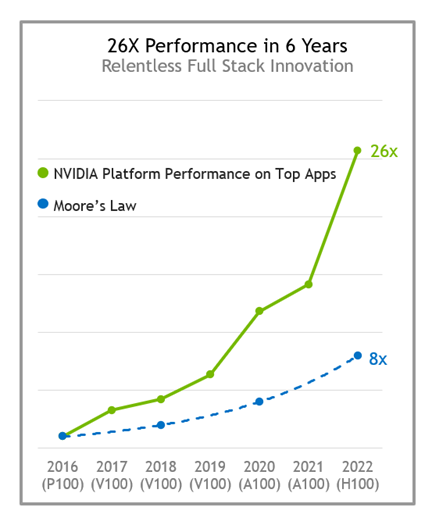
\includegraphics[scale=0.6]{nvidiaGraph.png}
        \cite{nvidia}
        \caption{A comparison of Nvidia hardware progress compared to Moore's law. The A100 GPU was used to train OpenAI's GPT-4. \cite{gpt4}}
    \end{figure}

    \item \textbf{Lack of regulations and restrictions.} There are currently no restrictions on the development of such technologies in the US, and the EU has introduced limited restrictions in the new AI act \cite{aiact}. There are obvious geopolitical incentives to allow the acceleration of GAI technologies, and open letters calling to pause giant AI experiments have failed to bring action \cite{fol}.
    \item \textbf{Profit incentives.} Such technologies are applicable across a huge spectrum of high-level tasks. There was 14 billion dollars in funding in 2023 towards GAI technologies.
\end{itemize}
\subsection{A Look at the SOTA}
 A big part of the motivation for such a project comes from the unbelievable progress and ability of current GAI models, and how we might attempt to improve their detection. Therefore, in this section we take a brief look into the current state-of-the-art in GAI. At the moment there are two dominant model types in the GAI world:
\begin{itemize}
    \item Transformer models, used for text generation
    \item Diffusion models, used for image and video generation
\end{itemize}
Transformers were initially designed for NLP tasks, but have proven to be incredibly versatile and scalable \cite{scaling}. Performance has increased linearly with model size, even as model sizes have increased to trillions of parameters. 
\begin{figure}[H]
    \centering
    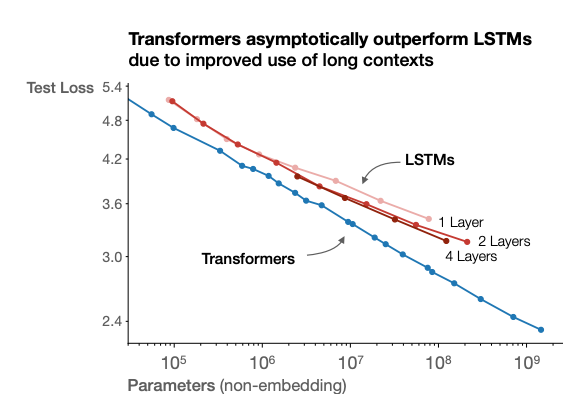
\includegraphics[scale=1]{linearScaling.png}
    \caption{Test loss (performance) against size (parameter count) of a model}
\end{figure}
\noindent SOTA for Transformers is currently Claude Opus, recently released by Anthropic. A few stats include Opus achieving 86.8\% on the MMLU (Undergraduate level multiple choice test) and 84.9\% on the HumanEval code benchmark \cite{opus}.
\\\\
Diffusion models gradually transform noise into a coherent image, based on learned data distributions. The SOTA is inherently more subjective in this area, but Midjourney version 5 is widely regarded as a front-runner in image generation. Midjourney can generate extremely detailed images from highly specific prompts.
\begin{figure}[H]
    \centering
    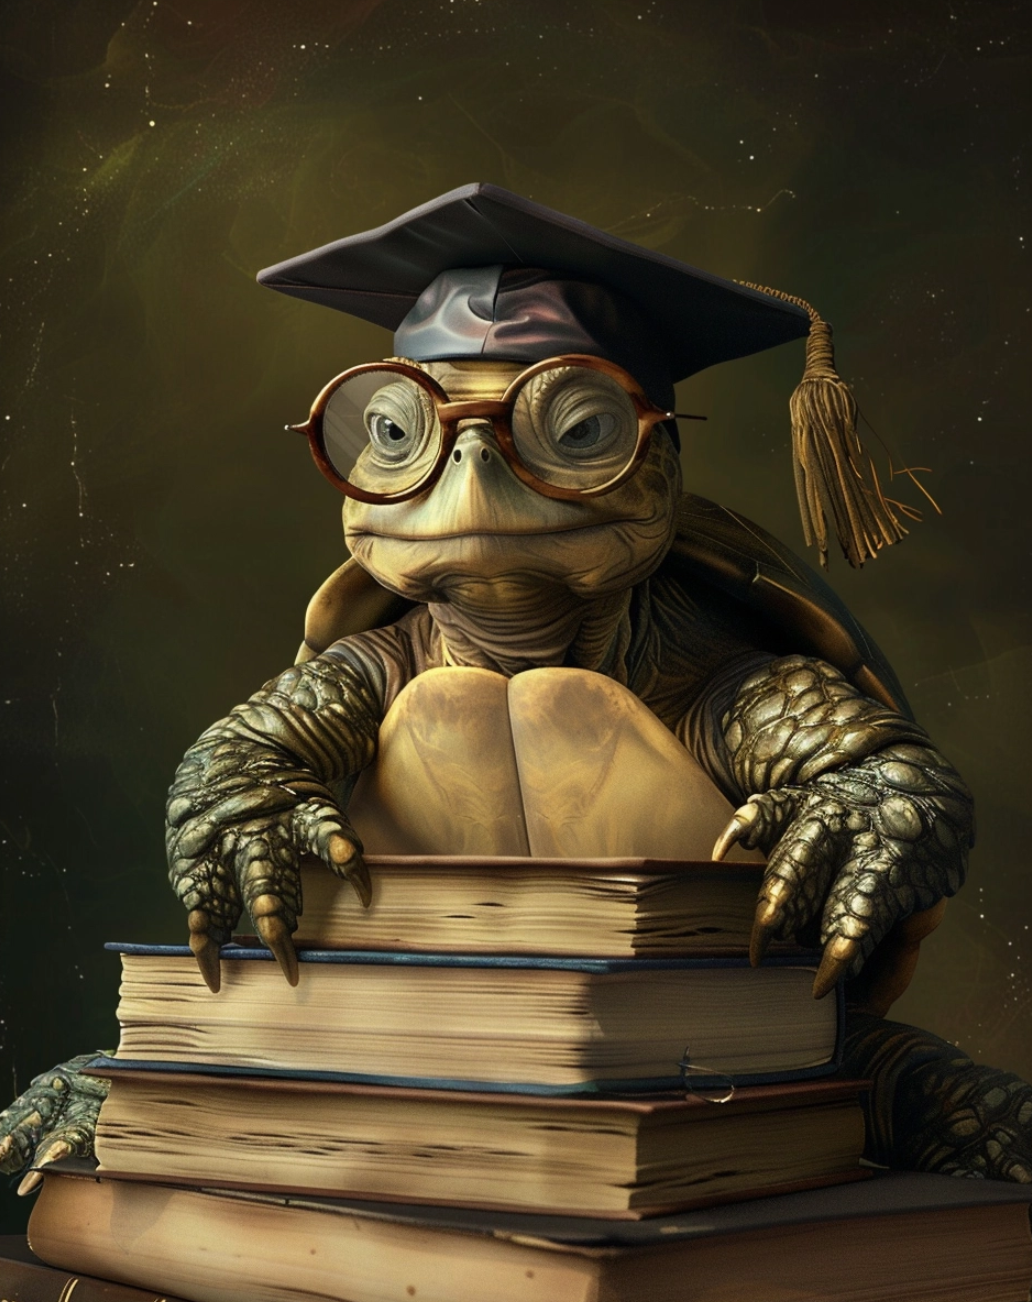
\includegraphics[scale=0.4]{turtle.png}
    \caption{Generated using Midjourney with the prompt: `A scholarly turtle wearing glasses and a graduation cap, sitting in front of a stack of books. He has a wise and contemplative expression, as if lost in philosophical thought'}
\end{figure}
\noindent SOTA in video generation is clearly Sora, a recently released model from OpenAI which took the industry by surprise. Essentially working by diffusion but on multiple frames, Sora can also take in highly specific prompts and output detailed and realistic videos. 
\begin{figure}[H]
    \centering
    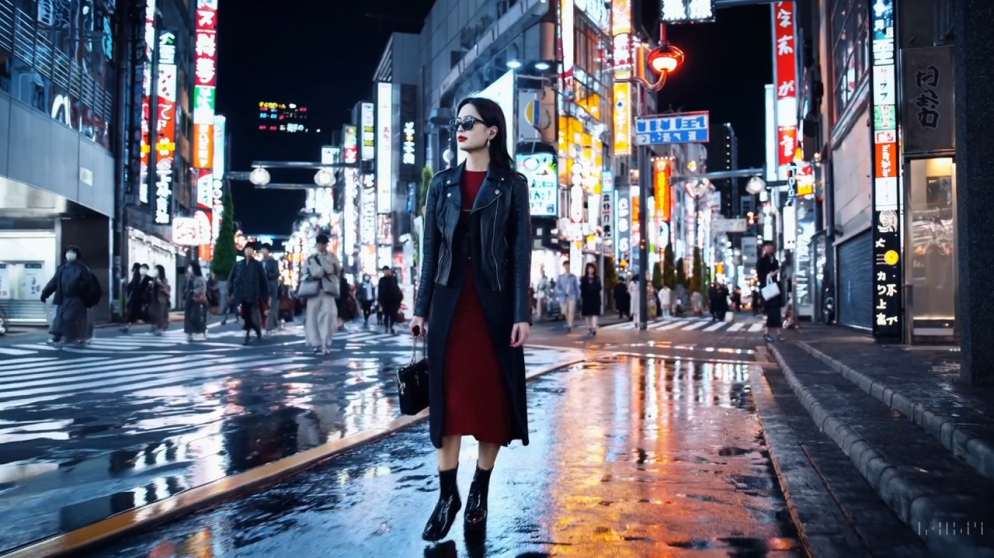
\includegraphics[scale=0.4]{sora.jpg}
    \caption{A frame from a Sora video, generated with the prompt: `A stylish woman walks down a Tokyo street filled with warm glowing neon and animated city signage. She wears a black leather jacket, a long red dress, and black boots, and carries a black purse. She wears sunglasses and red lipstick. She walks confidently and casually. The street is damp and reflective, creating a mirror effect of the colorful lights. Many pedestrians walk about.'}
\end{figure}
\subsection{Preserving Human Creativity}
The implication is that soon, we will be inundated with synthetic media and art. Whilst it is important to preserve human creations for philosophical reasons like maintaining the human identity, creative spirit and pride, there are two clearer motivators for building HumanMade:
\begin{enumerate}
    \item There will be free-market demand for authentic, human made creativity
    \item There is demand for GAI detection and tracking
\end{enumerate}
Expanding on the first - recent research (perhaps unsurprisingly) shows a clear bias in humans towards human made art \cite{anthropocentric}. In this study, participants in different groups were presented with the same piece of art, but labelled as either human made or AI made. These labels directly effected a participants' preference to buy the art, via biased perceptions of the creativity and awe they felt towards it.
\begin{figure}[H]
    \centering
    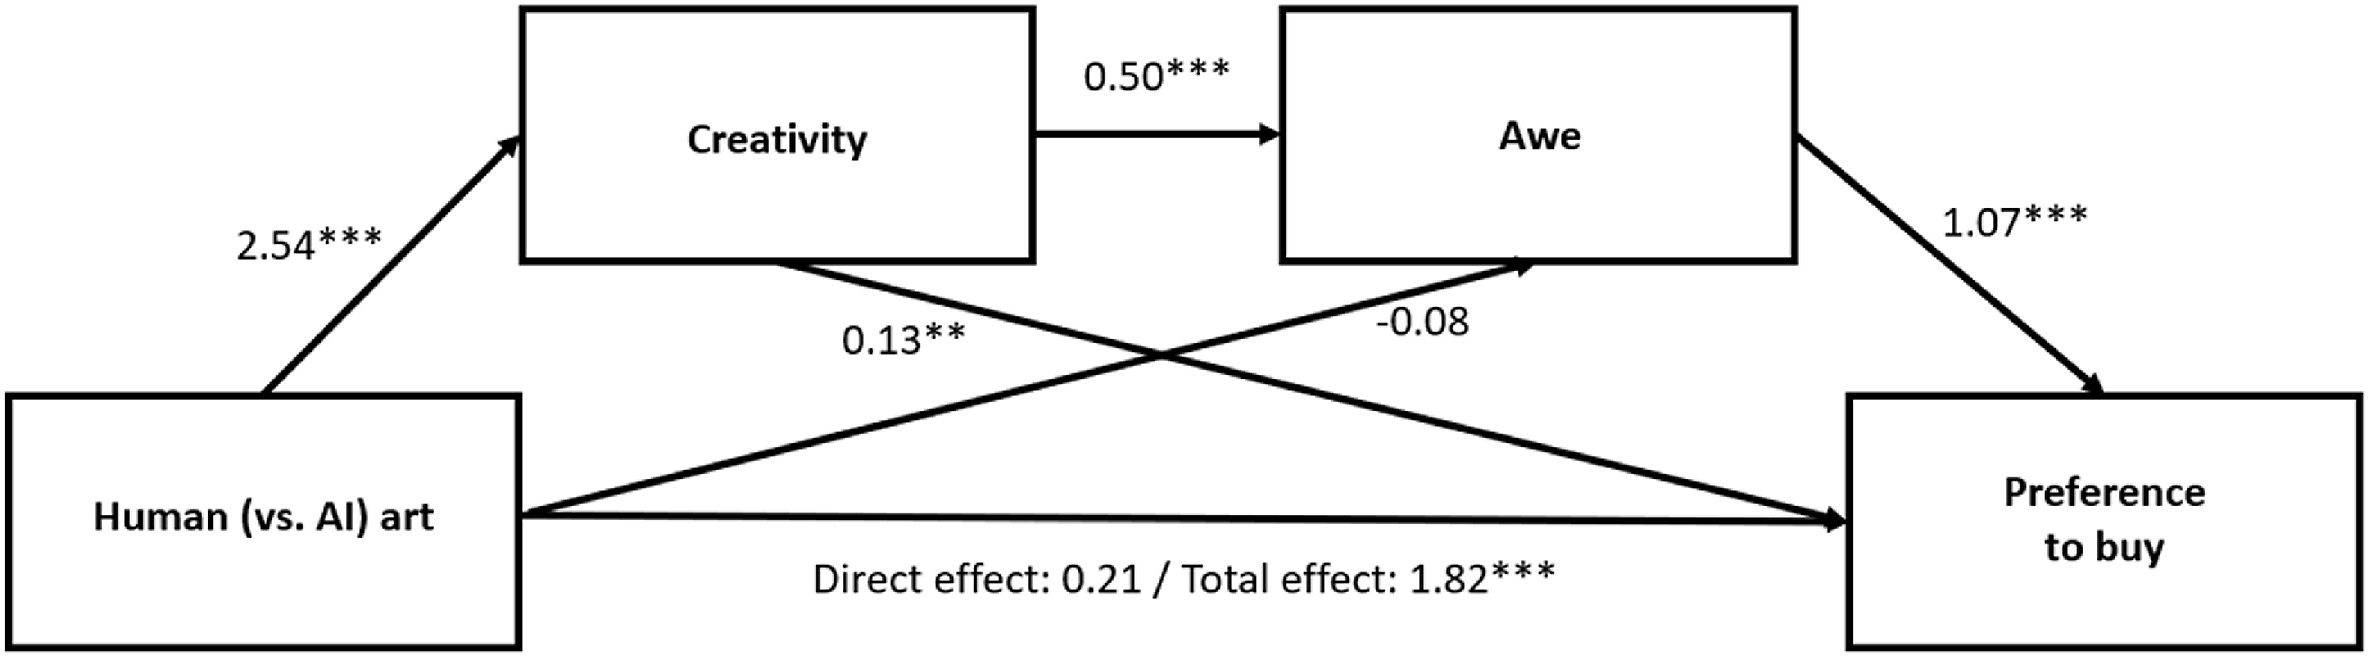
\includegraphics[scale=1]{biasDiagram.jpg}
    \caption{Indirect effect of human (vs. AI) art on preference to buy via perceived creativity and experienced awe.}
\end{figure}

\noindent On the second - tools which attempt to detect GAI are extremely popular (and for obvious reasons). For example GPTZero, a tool which attempts to detect AI generated text, has over 2.5 million users and partnerships with more than 100 organizations \cite{gptzero}. Industry-leading creative software developers Adobe have recently released Content Credentials, which is closer in spirit to what HumanMade is attempting. Both of these tools and more related systems will be further looked into subsequently.
\section{Background}
\subsection{Related systems}
We now look to analyse related systems and rate them out of 5 in three different categories - claimed capabilities, accuracy, and ease of use. This will give insight into what the best way to approach the development of HumanMade could be. In general, findings re-iterated the demand for a platform which does more than just attempt direct detection of AI. There were no holistic products with the aim of promoting human creativity.
\begin{table}[h]
    \centering
    \begin{tabular}{|M{3cm}|M{3cm}|M{3cm}|M{3cm}|}
    \hline
    System & Capabilities & Accuracy & Ease of Use \\ \hline 
    Adobe Content Credentials & 3 & 2 & 5\\
                           
\end{tabular}
\end{table}

\noindent Content credentials \cite{adobe} is advertised as, first and foremost, a way for creators to attach credit and usage details to their work, and second as a way to be transparent with AI generation. At the former it succeeds, however with the latter, content credentials only indicates the use of generation with regard to Adobe Firefly and other proprietary apps. This does not solve the issue of verifying any piece of AI generated content as specifically human made. Accuracy is poor as the system can easily be cheated - someone could screenshot a piece of digital work and then export it themselves. Ease of use is high as the feature is built right into industry leading apps used for content creation.

\begin{table}[h]
    \centering
    \begin{tabular}{|M{3cm}|M{3cm}|M{3cm}|M{3cm}|}
    GPTZero & 1 & 4 & 5\\
                           
\end{tabular}
\end{table}
\noindent GPTZero is a web interface that detects whether your pasted in text is AI generated or not. From testing by pasting in GPT-4 (the current state of the art for chatbots according to the widely used Huggingface arena leaderboard \cite{huggingface}) generated text, GPTZero performs fairly accurately, predicting 6/7 samples overwhelmingly correctly. GPTZero is a paid service beyond 7 free scans, and does not support any other types of content. Other systems tested perform at or worse than GPTZero.
\begin{table}[h]
    \centering
    \begin{tabular}{|M{3cm}|M{3cm}|M{3cm}|M{3cm}|}
    Sensity & 4 & 4 & 5\\
    \hline
\end{tabular}
\end{table}
\\\noindent Sensity is a leader in deepfake detection and has a high accuracy according to a recent study \cite{sensityStudy}. It has API, SDK and UI offerings.
\subsection{Issues with Direct Detection}
Despite accuracy scores for related systems initially looking positive, research shored up bigger picture concerns when considering a direct detection approach. GAI systems are improving at such a rapid pace that it will likely be impossible to keep up with them. 
\\\\Sensity mentions on their site, `As AI technology advances, new and more sophisticated techniques for generating realistic images emerge. Keeping up with these developments requires constant innovation and vigilance.' \cite{sensityBlog}. Sensity uses mainly ML techniques to identify GAI content \cite{sensityBlog}, and so of course the detection model is only as up-to-date as the data used to train it. When a cutting edge GAI model like Sora drops, content remains undetectable until detection techniques catch up again (assuming it is even possible for them to do so). \\\\Further, during the course of this third year project, Humbot was released \cite{humbot}. Humbot `humanizes' AI text to avoid detection by tools like GPTZero and Turnitin. Upon initial testing (\ref{fig:humbotFig}), Humbot works very well, and there are many examples and reviews of functionality on their site.  
\begin{figure}[h]
    \centering
    \begin{minipage}{0.45\textwidth}
        \centering
        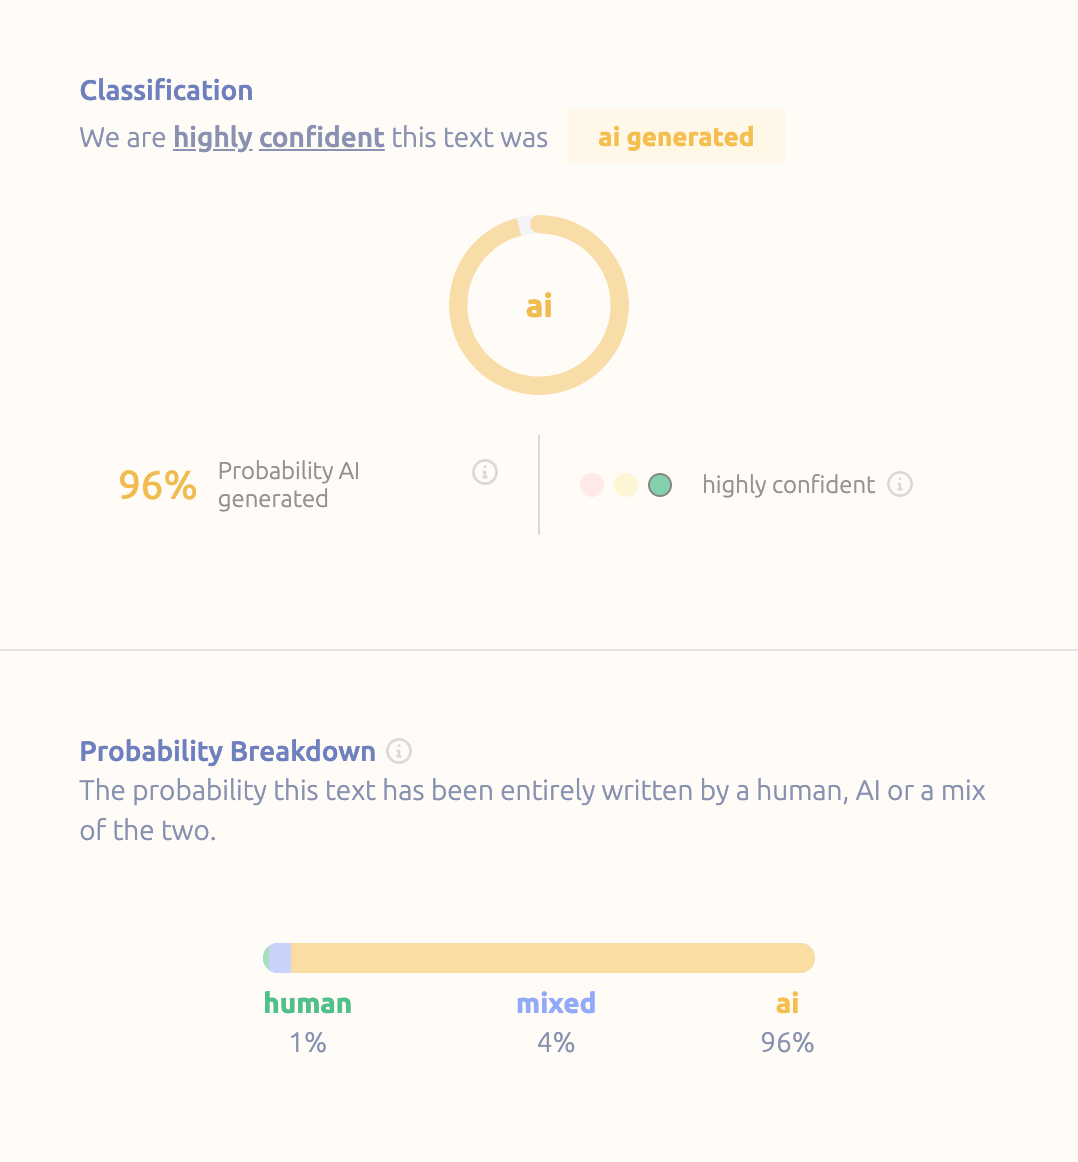
\includegraphics[width=\textwidth]{humbot2.png}
        \caption{GPTZero classification before using Humbot}
    \end{minipage}\hfill
    \begin{minipage}{0.45\textwidth}
        \centering
        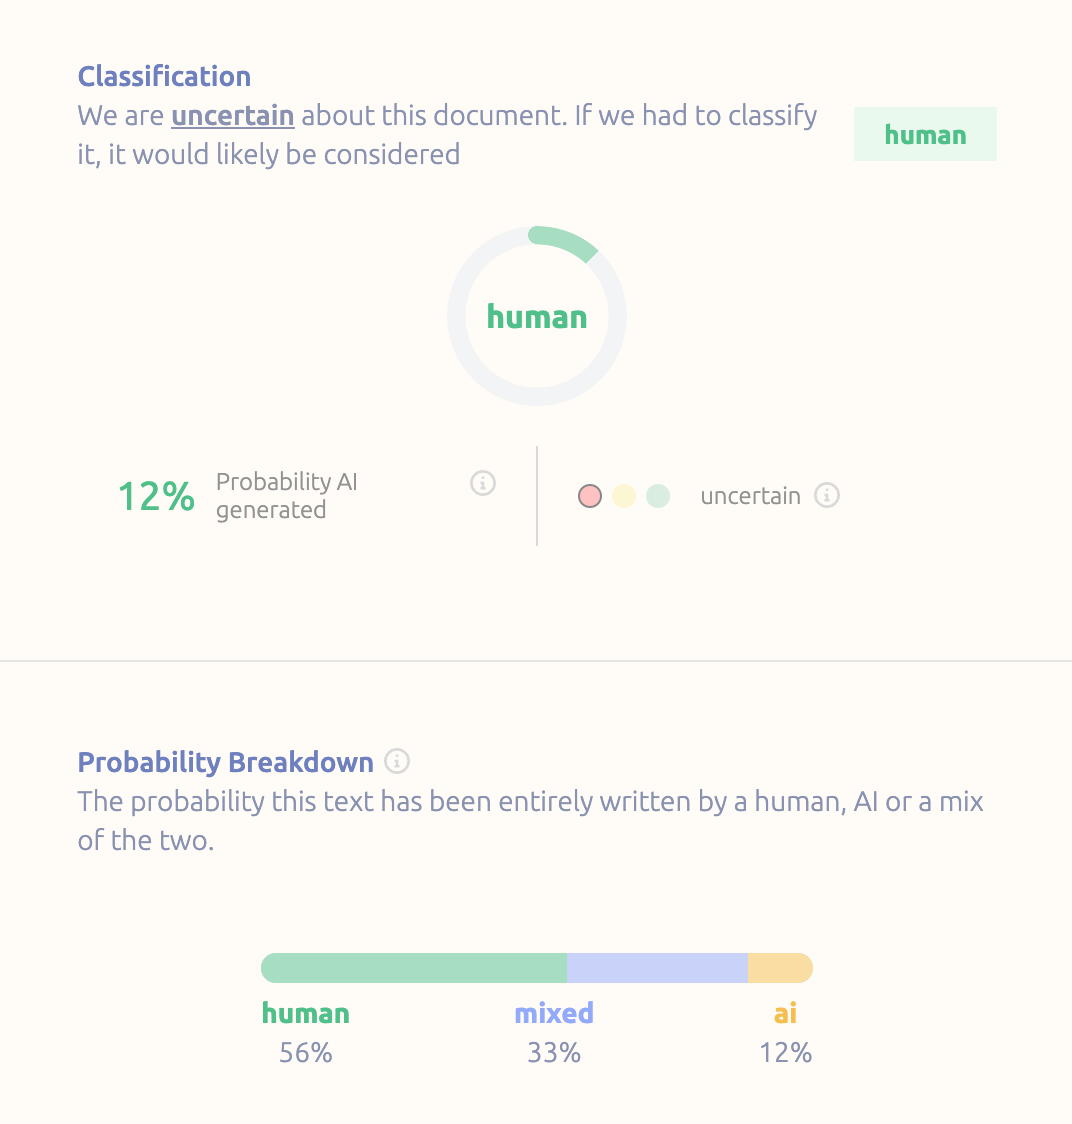
\includegraphics[width=\textwidth]{humbot1.png}
        \caption{Classification after using Humbot}
        \label{fig:humbotFig}
    \end{minipage}
\end{figure}

\section{Objectives}
After adequate research and analysis of the industry, the core objectives for HumanMade were then:
\begin{itemize}
    \item Creation of an intuitive and modern web app, allowing users to view and support human-made creations
    \item An easy way for creators to document their project and creative process to the app
    \item A way to ensure uploaded content is tamper-proof and traceable to a the author
\end{itemize}
\section{Design}
\subsection{Initial Design Ideas}
Initially, to circumvent the extensive issues with direct detection detailed previously, but to still allow for seamless and automatic verification, HumanMade was to work on an `evidence collection' basis. Evidence relating to the creative process itself would be collected, with the hope that this would give enough of a holistic input to whatever (likely ML) model was to be used to decide whether a creation was human or AI generated. Upon starting the project, there were some large caveats with this approach:
\subsubsection{Issues}
\begin{itemize}
    \item Data collection for training would be long \& an unproductive use of time. There were no existing datasets for my purpose.
    \item Data collected would be messy, with few consistent patterns. `Evidence' could have included screen recordings, screenshots, timelapses, etc. There would not have been many consistent underlying features or patterns to learn to make a fully automated ML approach work well.
    \item Not actually avoiding the fundamental issues stemming from direct detection. At some point, GAI technologies would probably get so good that they would be able to generate the evidence being used to identify human made creations. This leads to a further philosophical point detailed later, but it was clear a more holistic approach would be required.
\end{itemize}
\subsection{Final Design}
The final design relies on some partially automated verification to give users an easier time identifying what might be human made, but the main approach revolves around the key concept of a progression timeline. 
\begin{itemize}
    \item Each progression timeline consists of `commits', akin to a git branch.
    \item Each creator-defined commit consists of files, a description, a percentage of completion, and an icon to denote whether AI was used.
    \item There is a simple interface to make any commit tamper-proof and traceable.
    \item There is a command line interface for easy publishing to the progress timeline for creatives.
\end{itemize}
\subsubsection{Advantages}
This approach had some inherent advantages, addressing the systemic issues we would see when attempting direct detection.
\begin{itemize}
    \item Generative AI has a very obvious `diffusion' progression. An image of pure noise is slowly transformed into the final output. This would be easy to spot on a progress timeline.
    \item The approach allows the community to decide the level of AI involvement in a creation they are comfortable with, as this is clearly a gray area. Certain AI tools which simply help a human creator be more effective in creating may not be inherently negative.
    \item The approach sidesteps the `arms race' between AI detectors and AI generators by allowing the community to decide for themselves what they think constitutes a human made creation. The best neural network detection algorithm to use to achieve the aims of human made is by necessity that of the human brain.
    \begin{figure}[h]
        \centering
        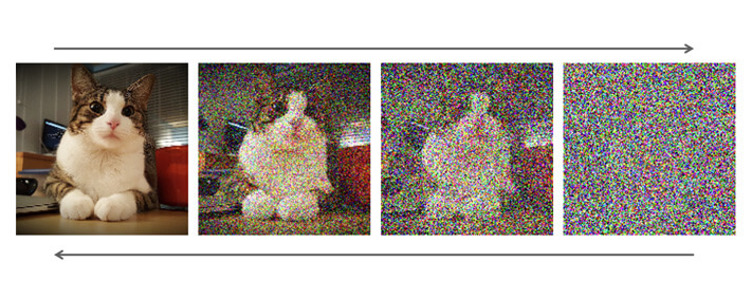
\includegraphics[scale=0.3]{catDiffusion.jpg}
        \caption{An example of the diffusion progression when generating a photo of a cat \cite{cat}.}
    \end{figure}
\end{itemize}
\section{Development}
\subsection{Architecture \& Tech Stack}
\subsection{Development Areas}
\subsubsection{Web App}
\subsubsection{Blockchain}
\subsubsection{Command Line Interface}
\subsection{Testing}

\section{Conclusions}
- evulation, process of production, lessons learnt, further work, limitations and contributoins

\section{Project Management}

\section{Philosophy of ito}
\newpage
\bibliography{finalReport}

\end{document}